\documentclass{article}

\usepackage[english]{babel}
\usepackage[utf8]{inputenc}
\usepackage{amsmath,amssymb}
\usepackage{parskip}
\usepackage{graphicx}
\usepackage{listings}
\usepackage{float}
\lstset{
    numbers=left, 
    numberstyle= \tiny, 
    keywordstyle= \color{ blue!70},
    commentstyle= \color{red!50!green!50!blue!50}, 
    frame=shadowbox, % 阴影效果
    rulesepcolor= \color{ red!20!green!20!blue!20} ,
    escapeinside=``, % 英文分号中可写入中文
    xleftmargin=2em,xrightmargin=2em, aboveskip=1em,
    framexleftmargin=2em,
    breaklines=true,
    language=Python
} 
% Margins
\usepackage[top=2.5cm, left=3cm, right=3cm, bottom=4.0cm]{geometry}
% Colour table cells
\usepackage[table]{xcolor}

% Get larger line spacing in table
\newcommand{\tablespace}{\\[1.25mm]}
\newcommand\Tstrut{\rule{0pt}{2.6ex}}         % = `top' strut
\newcommand\tstrut{\rule{0pt}{2.0ex}}         % = `top' strut
\newcommand\Bstrut{\rule[-0.9ex]{0pt}{0pt}}   % = `bottom' strut

%%%%%%%%%%%%%%%%%
%     Title     %
%%%%%%%%%%%%%%%%%
\title{CSCI803 Assignment}
\author{Yao Xiao \\ SID 2019180015}
\date{\today}

\begin{document}
\maketitle

%%%%%%%%%%%%%%%%%
%   Problem 1   %
%%%%%%%%%%%%%%%%%
\section*{Result Analysis}
To better analyze the results, I customized a set of input data to compare with the data already provided.

\begin{figure}[H]
    \caption{Output of ass2-sample-input}
    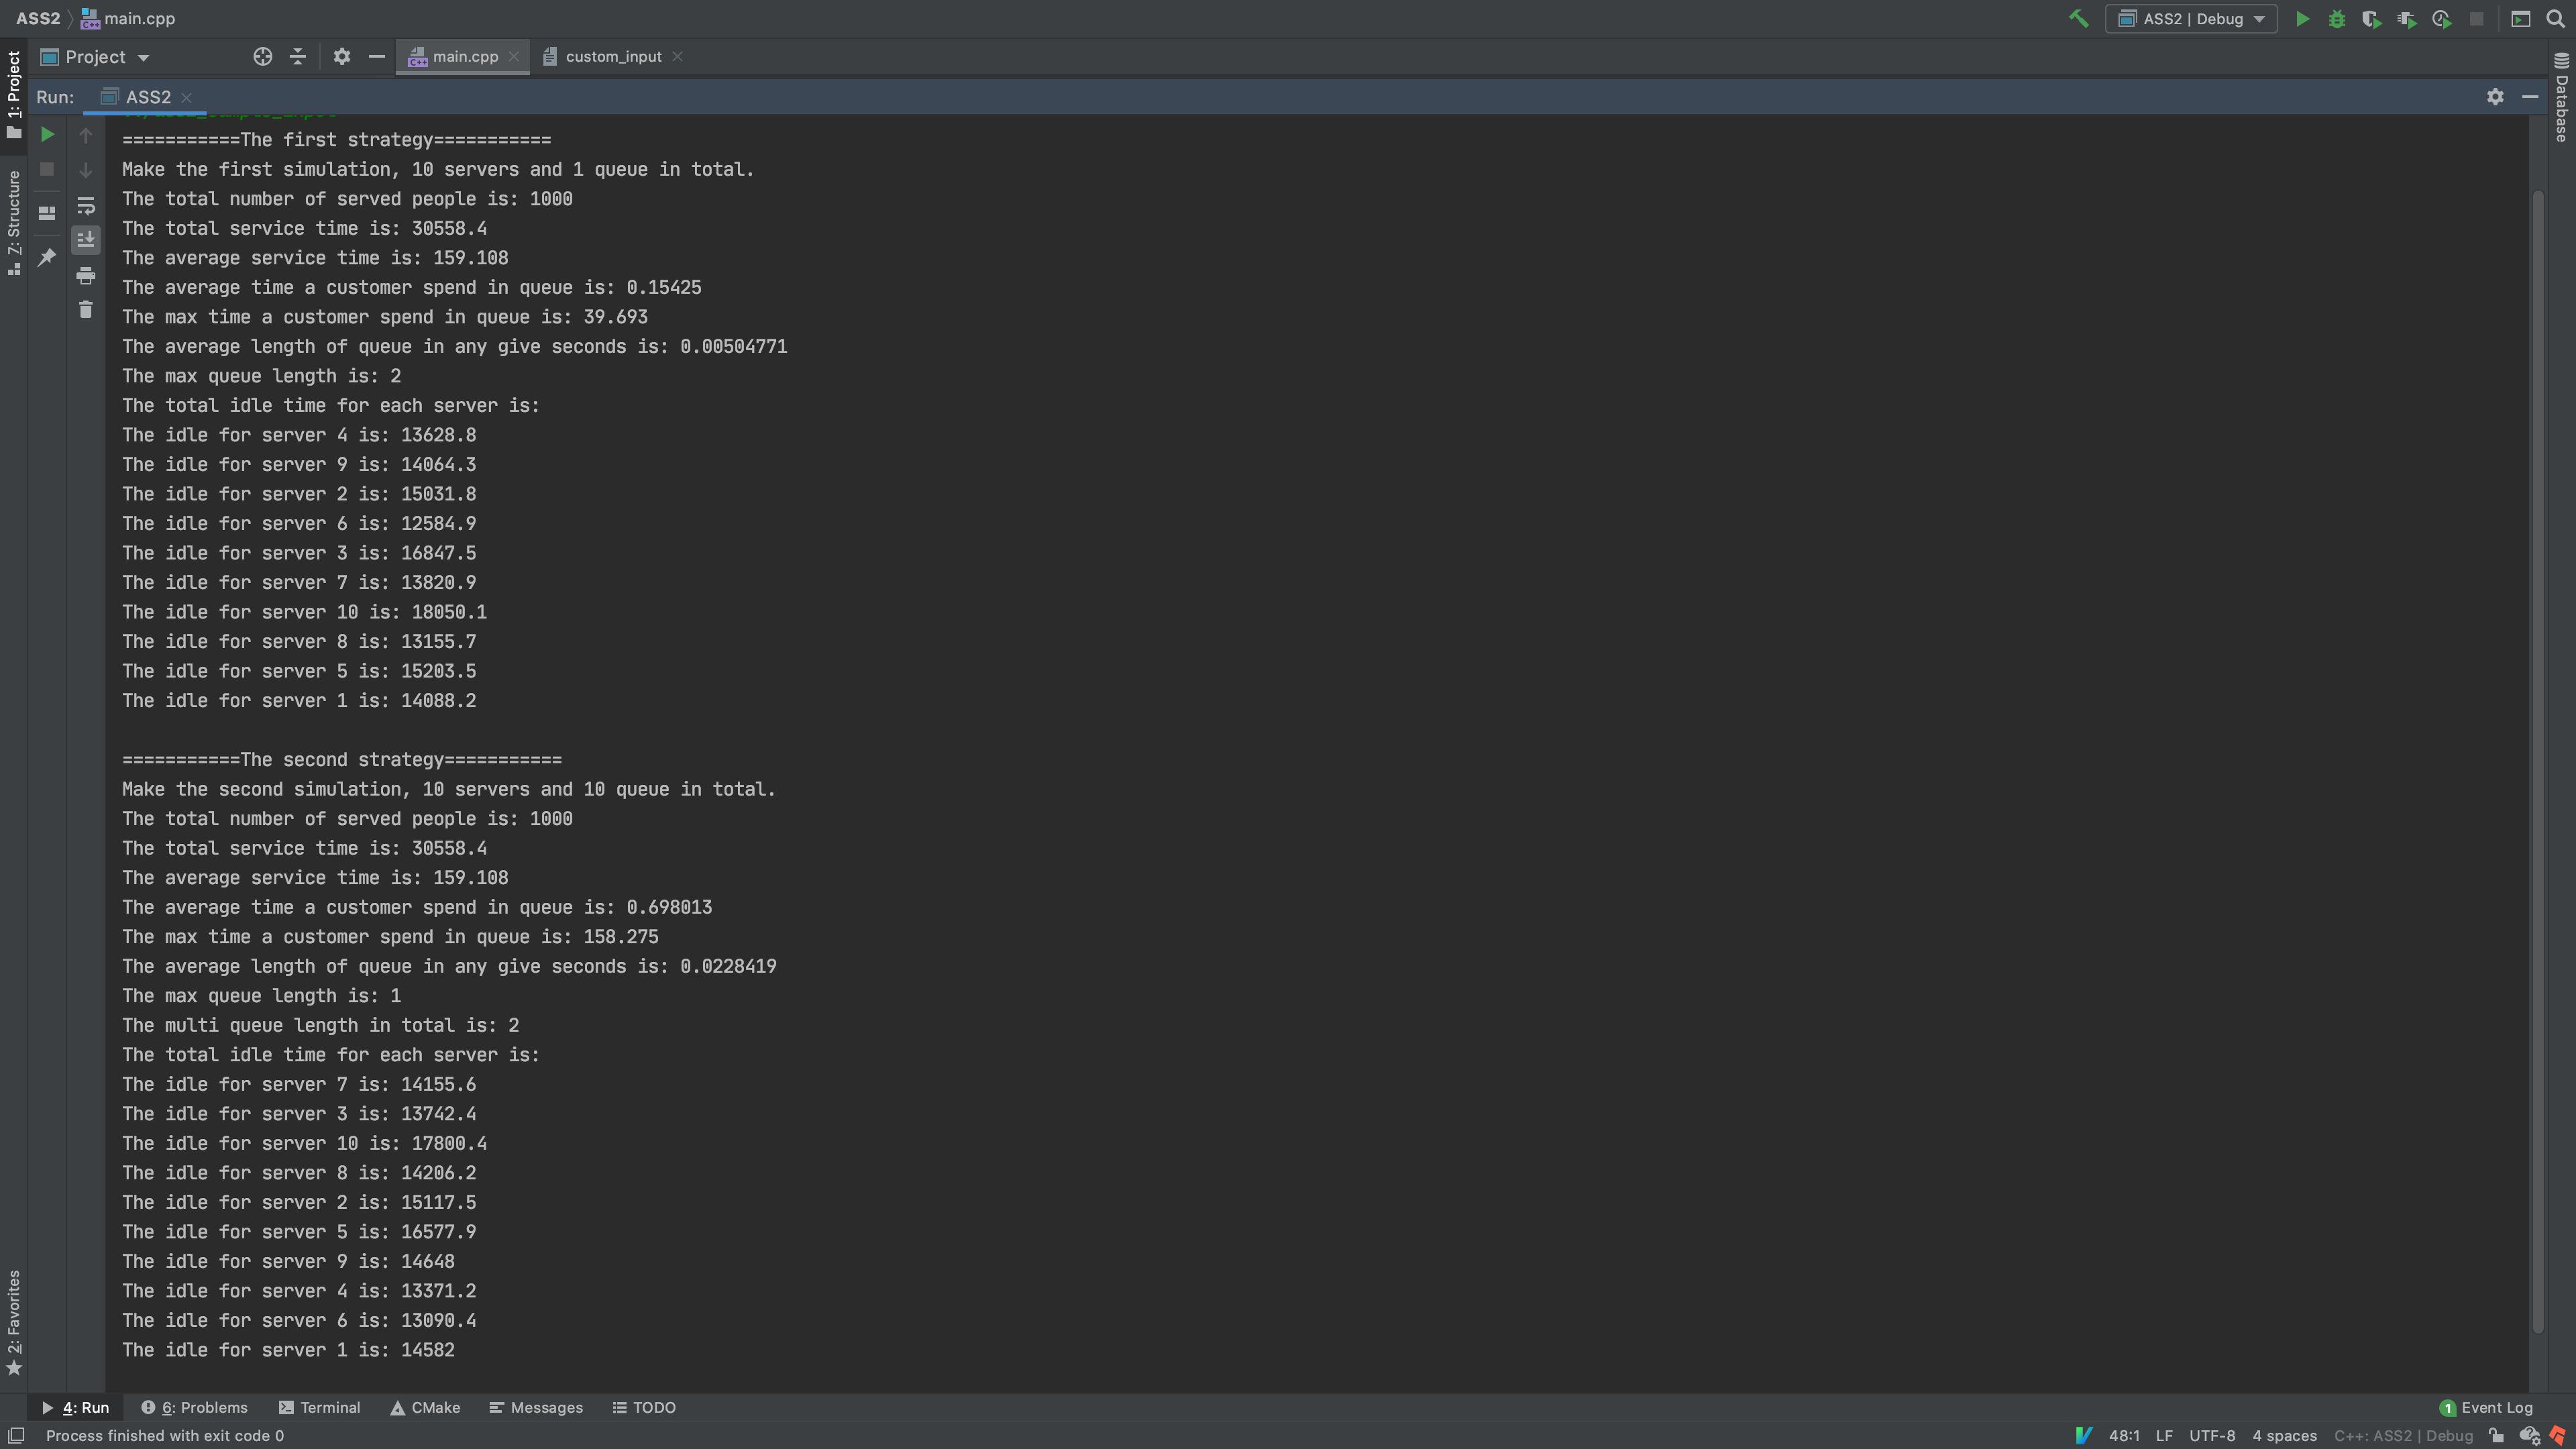
\includegraphics[width=1\textwidth]{Fig1}
\end{figure}

\begin{figure}[H]
    \caption{Output of custom-input}
    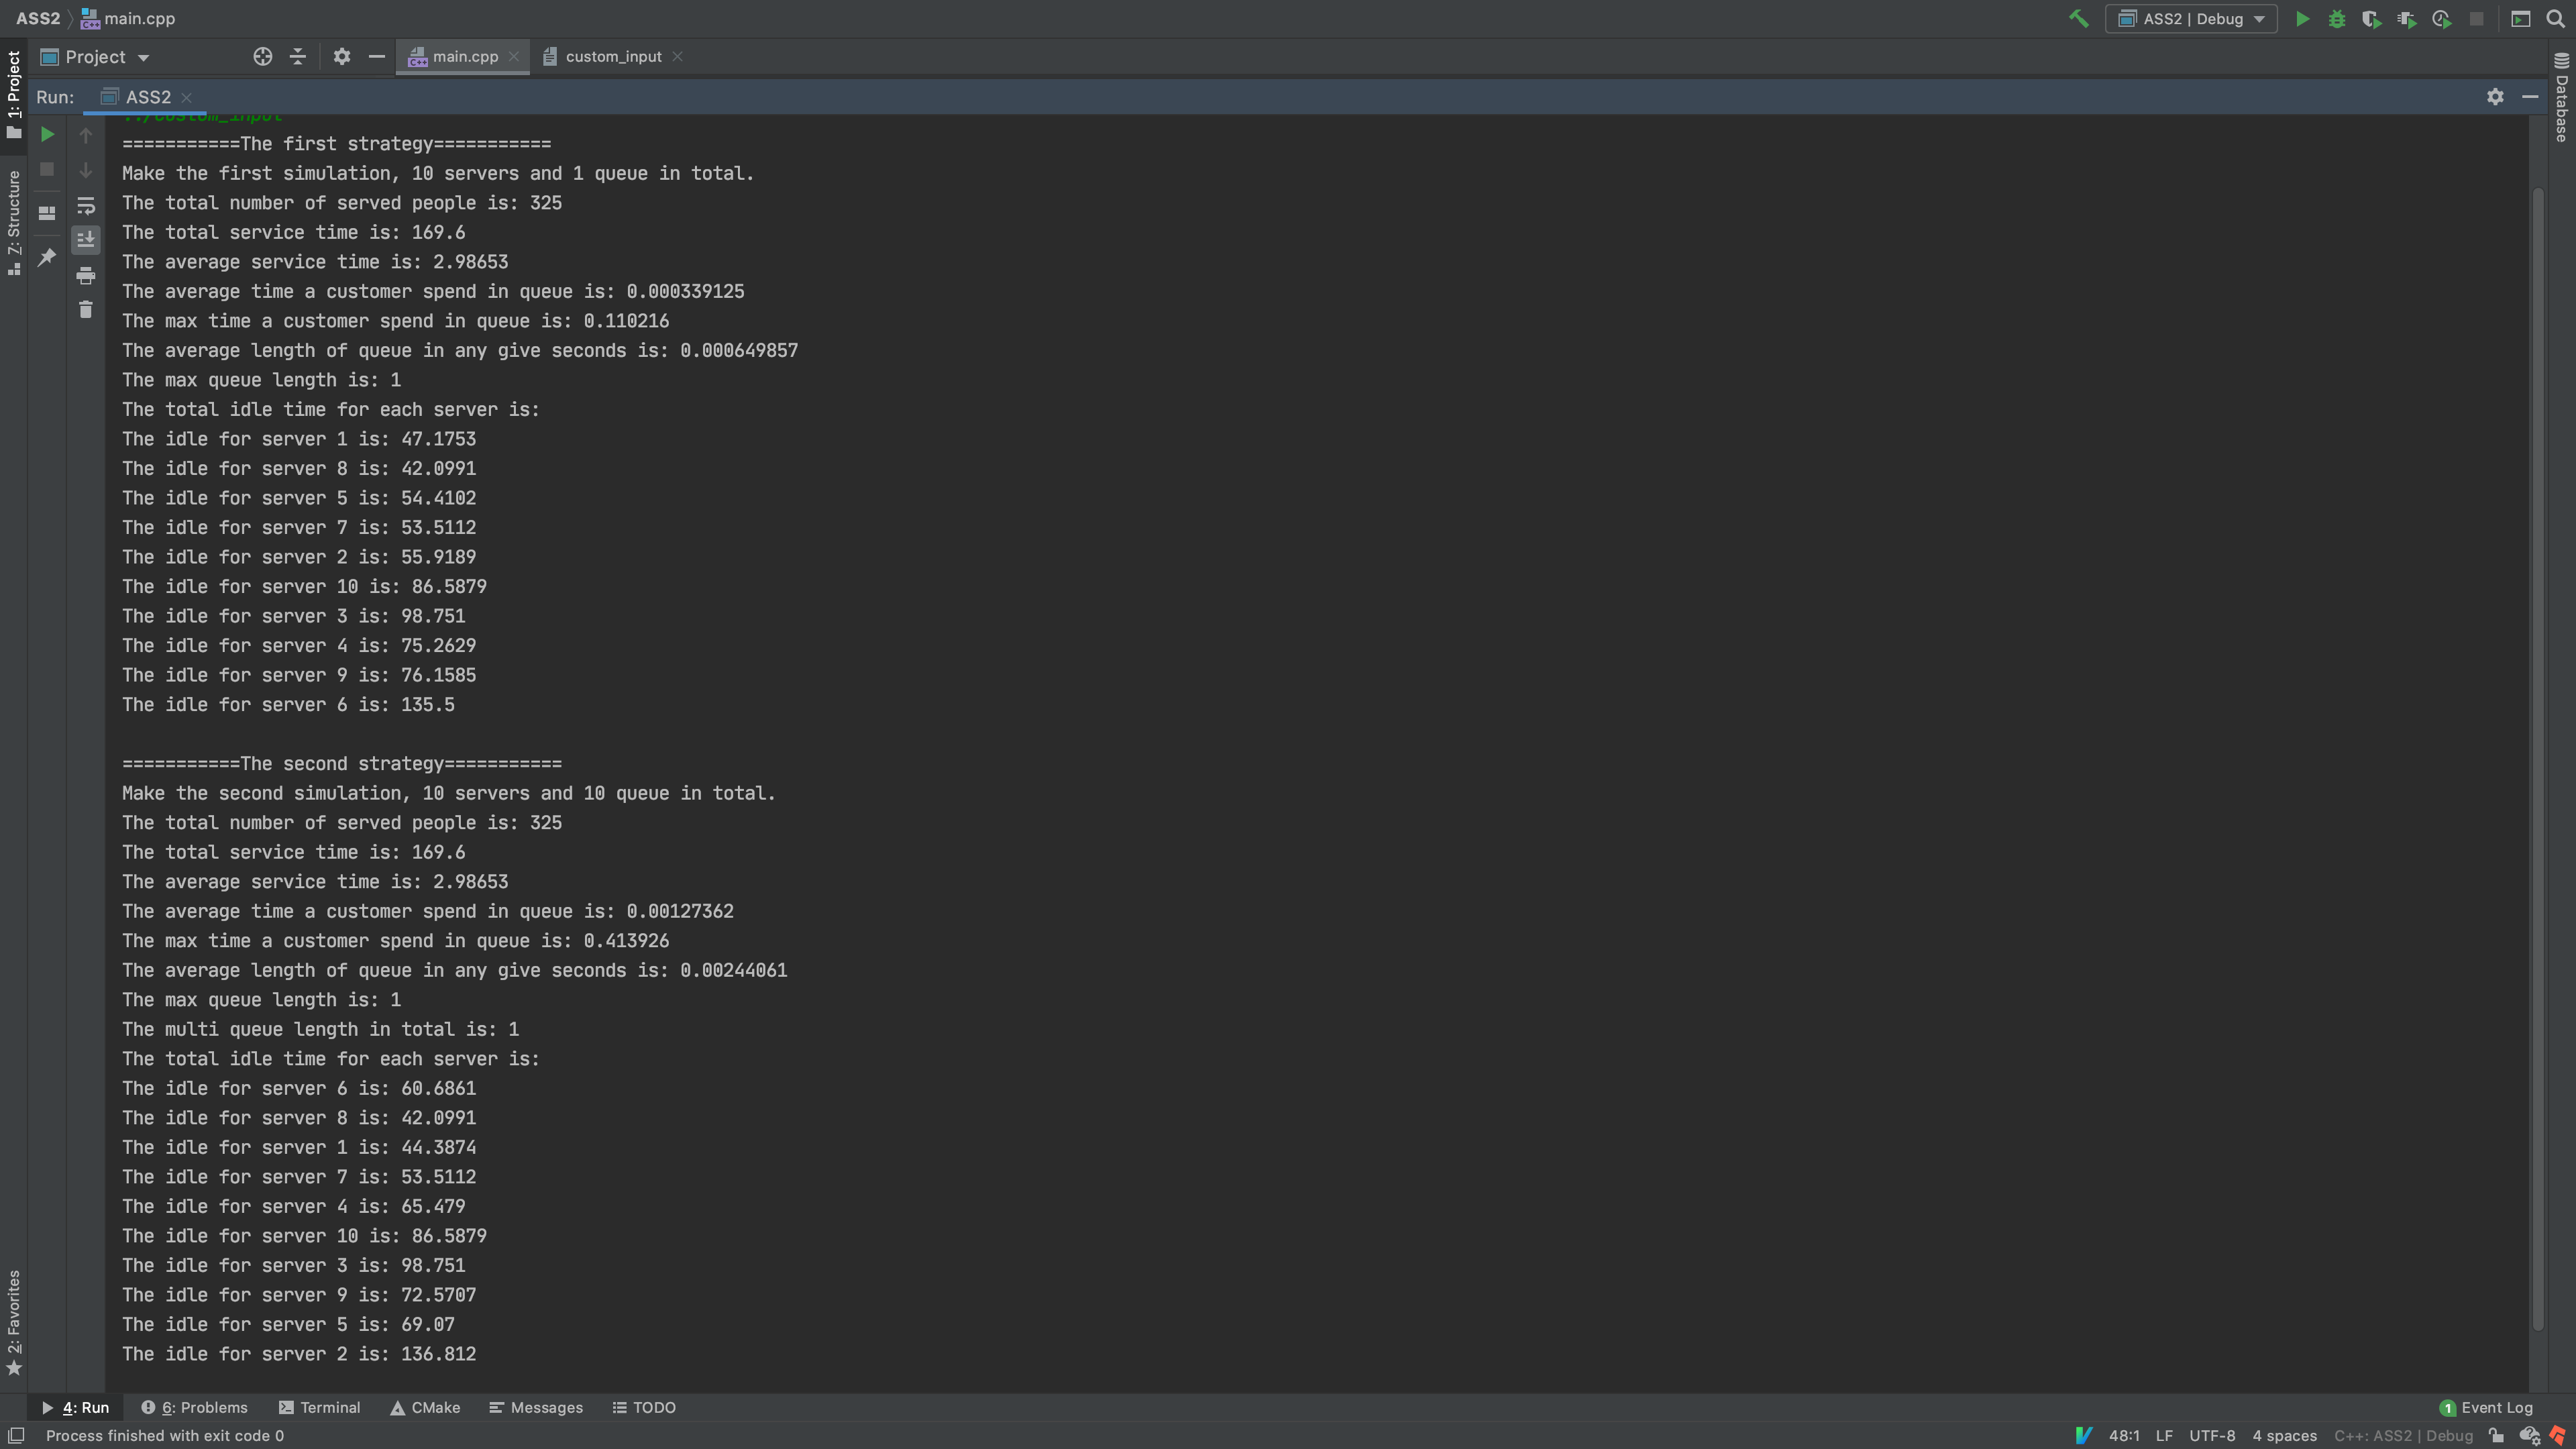
\includegraphics[width=1\textwidth]{Fig2}
\end{figure}


It can be seen that whether it is a custom data set or a data set that has been provided, in addition to the service time and average service time of the strategy 1, the service time and average service time are consistent with the strategy 2, the time each customer spends in the queue, the maximum time the customer is in the queue, and the average queue length is lower than strategy two, and for the idle time of each server, the idle time of each server in strategy one on average is also lower than strategy two which each customer spends a little bit more time in the queueon.

Taken together, strategy one is more efficient than strategy two





\end{document}
